%\section{Introduction}
%During the last decade, social video streaming for targeted audiences have seen a huge boom with applications like Twitch.tv, Periscope, Meerkat along with the traditional YouTube \& Facebook live and similar other personalized live streaming services~\cite{wang2016anatomy}. Live broadcasts over such platforms have increased many-folds during the recent COVID-19 pandemic due to over-the-top (OTT) services like online live broadcast of classroom lectures to the students\footnote{\url{https://www.nokia.com/blog/network-traffic-insights-time-covid-19-march-23-29-update/} (Accessed: \today)}. Many existing studies indicate that live streaming of popular events, such as a live cricket or football match, creates multiple traffic bottlenecks in the network, particularly at the Internet gateways of private organizational networks or Internet Service Providers (ISP)~\cite{yan2018understanding}. Consequently, a question arises -- how can we prevent traffic bottlenecks in the Internet while allowing high definition video streaming to millions of users? 

In the previous chapters, we have analyzed the online video streaming systems and developed a way to reduce the energy consumption while streaming online videos. In this chapter, we consider a class of live but non-interactive streaming applications, where the video is broadcast to a set of targeted audiences over social streaming applications. Social streaming applications many-a-times form communities which are localized, forming one or more geographical clusters~\cite{wang2016anatomy}. We utilize this localized community formations among live streaming viewers to construct one or more playback coalitions, as shown in \fig\ref{fig:chap06:flsd}. The coalition members share a common network gateway (such as an organizational local network gateway or the service gateway for a cellular core network) to connect to the Internet, however, there are direct high-speed local connections among the coalition members (like LAN connections or cellular device-to-device connections). It can be noted that such a coalition can be formed based on the principles of \textit{Application-Layer Traffic Optimization} (ALTO), where an ALTO server can provide the locality information of video players without requiring any explicit network or device firmware change. The coalition members collectively download the video from the content provider based on an adaptive bitrate streaming (ABR) strategy, such as dynamic adaptive streaming over HTTP (DASH).  The clients in a coalition collectively decide the adaptive playback rate and share data-download loads among themselves maintaining the playback synchronization. 
\begin{figure}[!ht]
    \centering
    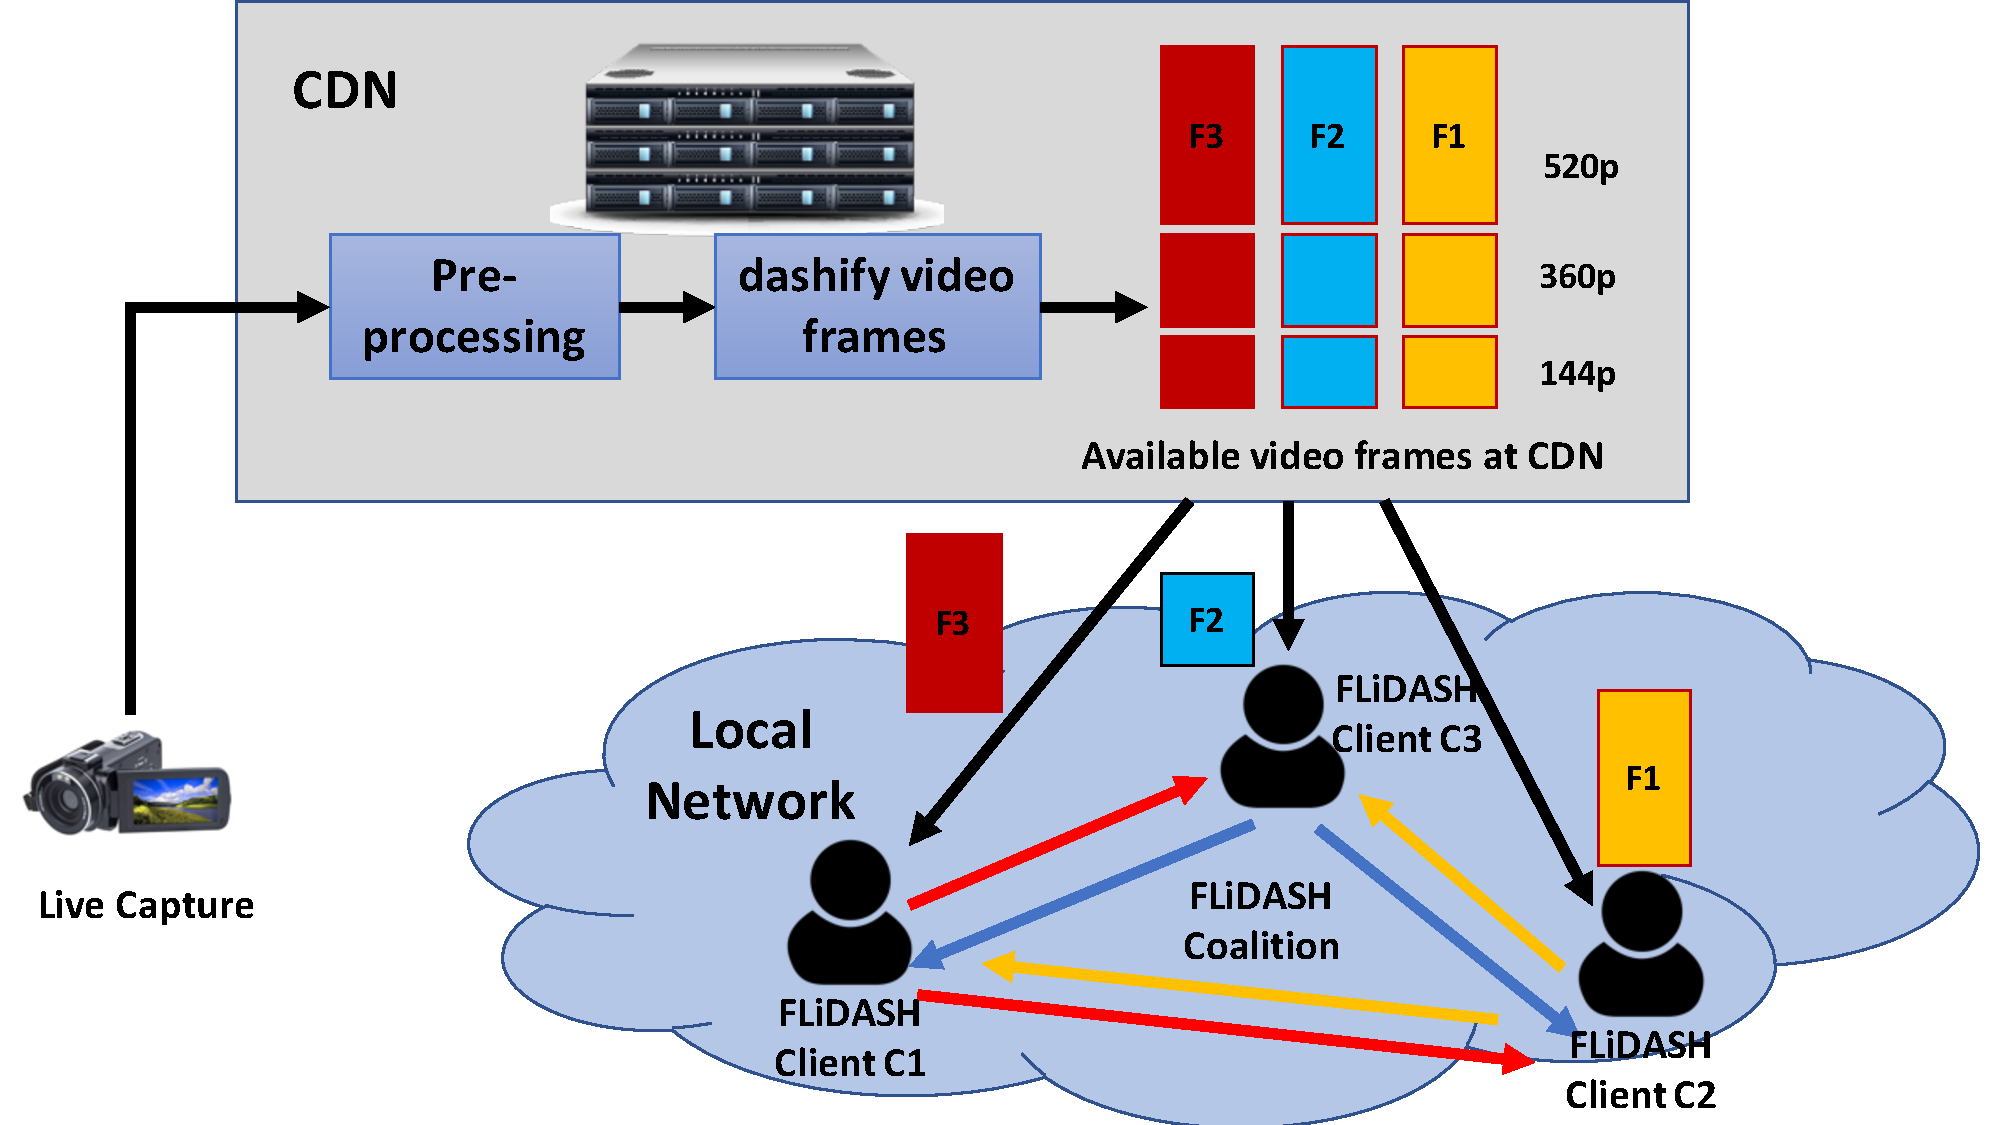
\includegraphics[width=0.8\linewidth]{img/flsd.pdf}
    \caption{Overview of \our: The clients under a local network create a coalition, every members of the coalition share the total download load.}
    \label{fig:chap06:flsd}
\end{figure}

However, developing such a system has multiple challenges. First, the coalition needs to be designed in a way such that downloading data directly from the content provider is costlier than sharing the data over the local network. Second, there should be a proper distribution of segment-wise data-download scheduling among the coalition members such that playback synchronization is not violated. A proper playback synchronization ensures that every player in the coalition should acquire the video segment $s_{i}$, either downloaded by itself or fetched from another coalition player through the direct local link, by the time it completes playing the previous video segment $s_{i-1}$; otherwise, there might be a rebuffering delay affecting the quality of experience (QoE). Third, the Internet bandwidth of individual players may vary over time; therefore, the coalition as a whole should schedule the video segment downloads among its members as well as decide the bitrate of every video segment based on the ABR principle.

Owing to the above challenges, we develop a coalition-based adaptive live streaming  called \textit{Federated Live Streaming over DASH} (\our) where the streaming clients or players form a dynamic coalition based on the network quality parameters and collectively stream a live video. We use the playback buffer statistics at individual streaming clients to develop a distributed mechanism for coalition formation with the help from a proximity server (which can be an ALTO server). The members of a coalition use a low-overhead gossip-based protocol for playback synchronization and takes following two decisions -- (1) scheduling the downloads of video segments among the coalition members based on their individual instantaneous network condition and the overall fairness criteria, and (2) bitrate of each video segments to optimize the overall QoE of the coalition. We use the following QoE objectives while making the above decisions -- (a) improve the overall video quality level, (b) improve the playback smoothness by reducing the quality fluctuations, (c) reduce rebuffering, and (d) improve fairness  among the coalition members in terms of the downloaded data share. We have implemented {\our} over an emulated environment and have thoroughly compared its performance with various other baselines. We observe that {\our} improves the overall QoE with less traffic overhead at the backbone network.

The rest of the chapter is organized as follows. 
